%**************************************%
%*    Generated from PreTeXt source   *%
%*    on 2019-08-30T10:14:27-06:00    *%
%*                                    *%
%*      https://pretextbook.org       *%
%*                                    *%
%**************************************%
\documentclass[oneside,10pt,]{article}
%% Custom Preamble Entries, early (use latex.preamble.early)
%% Default LaTeX packages
%%   1.  always employed (or nearly so) for some purpose, or
%%   2.  a stylewriter may assume their presence
\usepackage{geometry}
%% Some aspects of the preamble are conditional,
%% the LaTeX engine is one such determinant
\usepackage{ifthen}
%% etoolbox has a variety of modern conveniences
\usepackage{etoolbox}
\usepackage{ifxetex,ifluatex}
%% Raster graphics inclusion
\usepackage{graphicx}
%% Color support, xcolor package
%% Always loaded, for: add/delete text, author tools
%% Here, since tcolorbox loads tikz, and tikz loads xcolor
\PassOptionsToPackage{usenames,dvipsnames,svgnames,table}{xcolor}
\usepackage{xcolor}
%% Colored boxes, and much more, though mostly styling
%% skins library provides "enhanced" skin, employing tikzpicture
%% boxes may be configured as "breakable" or "unbreakable"
%% "raster" controls grids of boxes, aka side-by-side
\usepackage{tcolorbox}
\tcbuselibrary{skins}
\tcbuselibrary{breakable}
\tcbuselibrary{raster}
%% We load some "stock" tcolorbox styles that we use a lot
%% Placement here is provisional, there will be some color work also
%% First, black on white, no border, transparent, but no assumption about titles
\tcbset{ bwminimalstyle/.style={size=minimal, boxrule=-0.3pt, frame empty,
colback=white, colbacktitle=white, coltitle=black, opacityfill=0.0} }
%% Second, bold title, run-in to text/paragraph/heading
%% Space afterwards will be controlled by environment,
%% dependent of constructions of the tcb title
\tcbset{ runintitlestyle/.style={fonttitle=\normalfont\bfseries, attach title to upper} }
%% Spacing prior to each exercise, anywhere
\tcbset{ exercisespacingstyle/.style={before skip={1.5ex plus 0.5ex}} }
%% Spacing prior to each block
\tcbset{ blockspacingstyle/.style={before skip={2.0ex plus 0.5ex}} }
%% xparse allows the construction of more robust commands,
%% this is a necessity for isolating styling and behavior
%% The tcolorbox library of the same name loads the base library
\tcbuselibrary{xparse}
%% Hyperref should be here, but likes to be loaded late
%%
%% Inline math delimiters, \(, \), need to be robust
%% 2016-01-31:  latexrelease.sty  supersedes  fixltx2e.sty
%% If  latexrelease.sty  exists, bugfix is in kernel
%% If not, bugfix is in  fixltx2e.sty
%% See:  https://tug.org/TUGboat/tb36-3/tb114ltnews22.pdf
%% and read "Fewer fragile commands" in distribution's  latexchanges.pdf
\IfFileExists{latexrelease.sty}{}{\usepackage{fixltx2e}}
%% Footnote counters and part/chapter counters are manipulated
%% April 2018:  chngcntr  commands now integrated into the kernel,
%% but circa 2018/2019 the package would still try to redefine them,
%% so we need to do the work of loading conditionally for old kernels.
%% From version 1.1a,  chngcntr  should detect defintions made by LaTeX kernel.
\ifdefined\counterwithin
\else
    \usepackage{chngcntr}
\fi
%% Text height identically 9 inches, text width varies on point size
%% See Bringhurst 2.1.1 on measure for recommendations
%% 75 characters per line (count spaces, punctuation) is target
%% which is the upper limit of Bringhurst's recommendations
\geometry{letterpaper,total={340pt,9.0in}}
%% Custom Page Layout Adjustments (use latex.geometry)
%% This LaTeX file may be compiled with pdflatex, xelatex, or lualatex executables
%% LuaTeX is not explicitly supported, but we do accept additions from knowledgeable users
%% The conditional below provides  pdflatex  specific configuration last
%% The following provides engine-specific capabilities
%% Generally, xelatex is necessary non-Western fonts
\ifthenelse{\boolean{xetex} \or \boolean{luatex}}{%
%% begin: xelatex and lualatex-specific configuration
\ifxetex\usepackage{xltxtra}\fi
%% realscripts is the only part of xltxtra relevant to lualatex 
\ifluatex\usepackage{realscripts}\fi
%% fontspec package provides extensive control of system fonts,
%% meaning *.otf (OpenType), and apparently *.ttf (TrueType)
%% that live *outside* your TeX/MF tree, and are controlled by your *system*
%% fontspec will make Latin Modern (lmodern) the default font
\usepackage{fontspec}
%% 
%% Extensive support for other languages
\usepackage{polyglossia}
%% Set main/default language based on pretext/@xml:lang value
%% document language code is "en-US", US English
%% usmax variant has extra hypenation
\setmainlanguage[variant=usmax]{english}
%% Enable secondary languages based on discovery of @xml:lang values
%% Enable fonts/scripts based on discovery of @xml:lang values
%% Western languages should be ably covered by Latin Modern Roman
%% end: xelatex and lualatex-specific configuration
}{%
%% begin: pdflatex-specific configuration
\usepackage[utf8]{inputenc}
%% PreTeXt will create a UTF-8 encoded file
%% begin: font setup and configuration for use with pdflatex
\usepackage{lmodern}
\usepackage[T1]{fontenc}
%% end: font setup and configuration for use with pdflatex
%% end: pdflatex-specific configuration
}
%% Symbols, align environment, bracket-matrix
\usepackage{amsmath}
\usepackage{amssymb}
%% allow page breaks within display mathematics anywhere
%% level 4 is maximally permissive
%% this is exactly the opposite of AMSmath package philosophy
%% there are per-display, and per-equation options to control this
%% split, aligned, gathered, and alignedat are not affected
\allowdisplaybreaks[4]
%% allow more columns to a matrix
%% can make this even bigger by overriding with  latex.preamble.late  processing option
\setcounter{MaxMatrixCols}{30}
%%
%%
%% Division Titles, and Page Headers/Footers
%% titlesec package, loading "titleps" package cooperatively
%% See code comments about the necessity and purpose of "explicit" option
\usepackage[explicit, pagestyles]{titlesec}
%% Set global/default page style for document due
%% to potential re-definitions after documentclass
\pagestyle{plain}
%%
%% Create globally-available macros to be provided for style writers
%% These are redefined for each occurence of each division
\newcommand{\divisionnameptx}{\relax}%
\newcommand{\titleptx}{\relax}%
\newcommand{\subtitleptx}{\relax}%
\newcommand{\shortitleptx}{\relax}%
\newcommand{\authorsptx}{\relax}%
\newcommand{\epigraphptx}{\relax}%
%% Create environments for possible occurences of each division
%% Environment for a PTX "section" at the level of a LaTeX "section"
\NewDocumentEnvironment{sectionptx}{mmmmmm}
{%
\renewcommand{\divisionnameptx}{Section}%
\renewcommand{\titleptx}{#1}%
\renewcommand{\subtitleptx}{#2}%
\renewcommand{\shortitleptx}{#3}%
\renewcommand{\authorsptx}{#4}%
\renewcommand{\epigraphptx}{#5}%
\section[{#3}]{#1}%
\label{#6}%
}{}%
%% Environment for a PTX "subsection" at the level of a LaTeX "subsection"
\NewDocumentEnvironment{subsectionptx}{mmmmmm}
{%
\renewcommand{\divisionnameptx}{Subsection}%
\renewcommand{\titleptx}{#1}%
\renewcommand{\subtitleptx}{#2}%
\renewcommand{\shortitleptx}{#3}%
\renewcommand{\authorsptx}{#4}%
\renewcommand{\epigraphptx}{#5}%
\subsection[{#3}]{#1}%
\label{#6}%
}{}%
%% Environment for a PTX "subsubsection" at the level of a LaTeX "subsubsection"
\NewDocumentEnvironment{subsubsectionptx}{mmmmmm}
{%
\renewcommand{\divisionnameptx}{Subsubsection}%
\renewcommand{\titleptx}{#1}%
\renewcommand{\subtitleptx}{#2}%
\renewcommand{\shortitleptx}{#3}%
\renewcommand{\authorsptx}{#4}%
\renewcommand{\epigraphptx}{#5}%
\subsubsection[{#3}]{#1}%
\label{#6}%
}{}%
%%
%% Styles for six traditional LaTeX divisions
\titleformat{\chapter}[display]
{\normalfont\huge\bfseries}{\divisionnameptx\space\thechapter}{20pt}{\Huge#1}
[{\Large\authorsptx}]
\titleformat{name=\chapter,numberless}[display]
{\normalfont\huge\bfseries}{}{0pt}{#1}
[{\Large\authorsptx}]
\titlespacing*{\chapter}{0pt}{50pt}{40pt}
\titleformat{\section}[hang]
{\normalfont\Large\bfseries}{\thesection}{1ex}{#1}
[{\large\authorsptx}]
\titleformat{name=\section,numberless}[block]
{\normalfont\Large\bfseries}{}{0pt}{#1}
[{\large\authorsptx}]
\titlespacing*{\section}{0pt}{3.5ex plus 1ex minus .2ex}{2.3ex plus .2ex}
\titleformat{\subsection}[hang]
{\normalfont\large\bfseries}{\thesubsection}{1ex}{#1}
[{\normalsize\authorsptx}]
\titleformat{name=\subsection,numberless}[block]
{\normalfont\large\bfseries}{}{0pt}{#1}
[{\normalsize\authorsptx}]
\titlespacing*{\subsection}{0pt}{3.25ex plus 1ex minus .2ex}{1.5ex plus .2ex}
\titleformat{\subsubsection}[hang]
{\normalfont\normalsize\bfseries}{\thesubsubsection}{1em}{#1}
[{\small\authorsptx}]
\titleformat{name=\subsubsection,numberless}[block]
{\normalfont\normalsize\bfseries}{}{0pt}{#1}
[{\normalsize\authorsptx}]
\titlespacing*{\subsubsection}{0pt}{3.25ex plus 1ex minus .2ex}{1.5ex plus .2ex}
\titleformat{\paragraph}[hang]
{\normalfont\normalsize\bfseries}{\theparagraph}{1em}{#1}
[{\small\authorsptx}]
\titleformat{name=\paragraph,numberless}[block]
{\normalfont\normalsize\bfseries}{}{0pt}{#1}
[{\normalsize\authorsptx}]
\titlespacing*{\paragraph}{0pt}{3.25ex plus 1ex minus .2ex}{1.5em}
%%
%% Semantic Macros
%% To preserve meaning in a LaTeX file
%%
%% \mono macro for content of "c", "cd", "tag", etc elements
%% Also used automatically in other constructions
%% Simply an alias for \texttt
%% Always defined, even if there is no need, or if a specific tt font is not loaded
\newcommand{\mono}[1]{\texttt{#1}}
%%
%% Following semantic macros are only defined here if their
%% use is required only in this specific document
%%
%% Used to markup initialisms, text or titles
\newcommand{\initialism}[1]{\textsc{\MakeLowercase{#1}}}
\DeclareRobustCommand{\initialismintitle}[1]{\texorpdfstring{#1}{#1}}
%% Used for warnings, typically bold and italic
\newcommand{\alert}[1]{\textbf{\textit{#1}}}
%% Used for inline definitions of terms
\newcommand{\terminology}[1]{\textbf{#1}}
%% Division Numbering: Chapters, Sections, Subsections, etc
%% Division numbers may be turned off at some level ("depth")
%% A section *always* has depth 1, contrary to us counting from the document root
%% The latex default is 3.  If a larger number is present here, then
%% removing this command may make some cross-references ambiguous
%% The precursor variable $numbering-maxlevel is checked for consistency in the common XSL file
\setcounter{secnumdepth}{3}
%%
%% AMS "proof" environment is no longer used, but we leave previously
%% implemented \qedhere in place, should the LaTeX be recycled
\newcommand{\qedhere}{\relax}
%%
%% A faux tcolorbox whose only purpose is to provide common numbering
%% facilities for most blocks (possibly not projects, 2D displays)
%% Controlled by  numbering.theorems.level  processing parameter
\newtcolorbox[auto counter, number within=section]{block}{}
%%
%% This document is set to number PROJECT-LIKE on a separate numbering scheme
%% So, a faux tcolorbox whose only purpose is to provide this numbering
%% Controlled by  numbering.projects.level  processing parameter
\newtcolorbox[auto counter, number within=section]{project-distinct}{}
%% A faux tcolorbox whose only purpose is to provide common numbering
%% facilities for 2D displays which are subnumbered as part of a "sidebyside"
\newtcolorbox[auto counter, number within=tcb@cnt@block, number freestyle={\noexpand\thetcb@cnt@block(\noexpand\alph{\tcbcounter})}]{subdisplay}{}
%%
%% tcolorbox, with styles, for FIGURE-LIKE
%%
%% figureptx: 2-D display structure
\tcbset{ figureptxstyle/.style={bwminimalstyle, middle=1ex, blockspacingstyle, } }
\newtcolorbox[use counter from=block]{figureptx}[3]{lower separated=false, before lower={{\textbf{Figure~\thetcbcounter}\space#1}}, phantomlabel={#2}, unbreakable, parbox=false, figureptxstyle, }
%% tableptx: 2-D display structure
\tcbset{ tableptxstyle/.style={bwminimalstyle, middle=1ex, blockspacingstyle, coltitle=black, bottomtitle=2ex, titlerule=-0.3pt} }
\newtcolorbox[use counter from=block]{tableptx}[3]{title={{\textbf{Table~\thetcbcounter}\space#1}}, phantomlabel={#2}, unbreakable, parbox=false, tableptxstyle, }
%%
%% xparse environments for introductions and conclusions of divisions
%%
%% introduction: in a structured division
\NewDocumentEnvironment{introduction}{m}
{\notblank{#1}{\noindent\textbf{#1}\space}{}}{\par\medskip}
%% Localize LaTeX supplied names (possibly none)
\renewcommand*{\abstractname}{Abstract}
%% "tcolorbox" environment for a single image, occupying entire \linewidth
%% arguments are left-margin, width, right-margin, as multiples of
%% \linewidth, and are guaranteed to be positive and sum to 1.0
\tcbset{ imagestyle/.style={bwminimalstyle} }
\NewTColorBox{image}{mmm}{imagestyle,left skip=#1\linewidth,width=#2\linewidth}
%% For improved tables
\usepackage{array}
%% Some extra height on each row is desirable, especially with horizontal rules
%% Increment determined experimentally
\setlength{\extrarowheight}{0.2ex}
%% Define variable thickness horizontal rules, full and partial
%% Thicknesses are 0.03, 0.05, 0.08 in the  booktabs  package
\newcommand{\hrulethin}  {\noalign{\hrule height 0.04em}}
\newcommand{\hrulemedium}{\noalign{\hrule height 0.07em}}
\newcommand{\hrulethick} {\noalign{\hrule height 0.11em}}
%% We preserve a copy of the \setlength package before other
%% packages (extpfeil) get a chance to load packages that redefine it
\let\oldsetlength\setlength
\newlength{\Oldarrayrulewidth}
\newcommand{\crulethin}[1]%
{\noalign{\global\oldsetlength{\Oldarrayrulewidth}{\arrayrulewidth}}%
\noalign{\global\oldsetlength{\arrayrulewidth}{0.04em}}\cline{#1}%
\noalign{\global\oldsetlength{\arrayrulewidth}{\Oldarrayrulewidth}}}%
\newcommand{\crulemedium}[1]%
{\noalign{\global\oldsetlength{\Oldarrayrulewidth}{\arrayrulewidth}}%
\noalign{\global\oldsetlength{\arrayrulewidth}{0.07em}}\cline{#1}%
\noalign{\global\oldsetlength{\arrayrulewidth}{\Oldarrayrulewidth}}}
\newcommand{\crulethick}[1]%
{\noalign{\global\oldsetlength{\Oldarrayrulewidth}{\arrayrulewidth}}%
\noalign{\global\oldsetlength{\arrayrulewidth}{0.11em}}\cline{#1}%
\noalign{\global\oldsetlength{\arrayrulewidth}{\Oldarrayrulewidth}}}
%% Single letter column specifiers defined via array package
\newcolumntype{A}{!{\vrule width 0.04em}}
\newcolumntype{B}{!{\vrule width 0.07em}}
\newcolumntype{C}{!{\vrule width 0.11em}}
%% Footnote Numbering
%% Specified by numbering.footnotes.level
\counterwithin*{footnote}{section}
%% More flexible list management, esp. for references
%% But also for specifying labels (i.e. custom order) on nested lists
\usepackage{enumitem}
%% hyperref driver does not need to be specified, it will be detected
%% Footnote marks in tcolorbox have broken linking under
%% hyperref, so it is necessary to turn off all linking
%% It *must* be given as a package option, not with \hypersetup
\usepackage[hyperfootnotes=false]{hyperref}
%% configure hyperref's  \url  to match listings' inline verbatim
\renewcommand\UrlFont{\small\ttfamily}
%% Hyperlinking active in electronic PDFs, all links solid and blue
\hypersetup{colorlinks=true,linkcolor=blue,citecolor=blue,filecolor=blue,urlcolor=blue}
\hypersetup{pdftitle={Math 3410 Course Outline}}
%% If you manually remove hyperref, leave in this next command
\providecommand\phantomsection{}
%% If tikz has been loaded, replace ampersand with \amp macro
%% Custom Preamble Entries, late (use latex.preamble.late)
%% Begin: Author-provided packages
%% (From  docinfo/latex-preamble/package  elements)
%% End: Author-provided packages
%% Begin: Author-provided macros
%% (From  docinfo/macros  element)
%% Plus three from MBX for XML characters
\renewcommand{\abstractname}{Summary}
\newcommand{\lt}{<}
\newcommand{\gt}{>}
\newcommand{\amp}{&}
%% End: Author-provided macros
%% Title page information for article
\title{Math 3410 Course Outline}
\author{Sean Fitzpatrick\\
University of Lethbridge
}
\date{Fall 2019}
\begin{document}
%% Target for xref to top-level element is document start
\hypertarget{x:article:linalg-outline-2019}{}
\maketitle
\thispagestyle{empty}
\begin{abstract}
A second course in linear algebra. The Academic Calendar imposes the following topics:%
\par
Vector spaces over the real and complex numbers. Basis and dimension. Linear transformations. Change of basis. Gram-Schmidt orthogonalization. Eigenvectors and diagonalization. Canonical forms. Cayley-Hamilton Theorem.%
\par
Required prerequisite courses are Math 1410 (a first course in linear algebra), and Math 2000 (an introduction to proofs).%
\end{abstract}
%
%
\typeout{************************************************}
\typeout{Section 1 Welcome}
\typeout{************************************************}
%
\begin{sectionptx}{Welcome}{}{Welcome}{}{}{x:section:section-welcome}
\begin{introduction}{}%
Welcome to Math 3410 Linear Algebra, our most popular mathematics course at the 3000-level! Math 3410 is a second course in linear algebra. We will assume familiarity with basic computational procedures, like Gaussian elimination, matrix multiplication, etc.\@. We will take a dual-track approach in Math 3410, focusing on both theory and application. Theoretical content will demand some ability to write proofs. Applications will likely involve software and a small amount of coding.%
\par
Over the summer, the University of Lethbridge adopted an official recognition of our location on traditional Blackfoot territory. This acknowledgement also serves as a welcome message, and I am pleased to be able to include it here:%
\begin{quote}%
Oki, and welcome to the University of Lethbridge. Our University’s Blackfoot name is Iniskim, meaning Sacred Buffalo Stone. The University of Lethbridge acknowledges and deeply appreciates the Siksikaitsitapii peoples’ connection to their traditional territory. We, as people living and benefiting from Blackfoot Confederacy traditional territory, honour the traditions of people who have cared for this land since time immemorial. We recognize the diverse population of Aboriginal peoples who attend the University of Lethbridge and the contributions these Aboriginal peoples have made in shaping and strengthening the University community in the past, present, and in the future.%
\end{quote}
\end{introduction}%
%
%
\pagebreak
\typeout{************************************************}
\typeout{Subsection 1.1 Course staff}
\typeout{************************************************}
%
\begin{subsectionptx}{Course staff}{}{Course staff}{}{}{x:subsection:subsec-staff}
My name is \href{http://www.cs.uleth.ca/\~fitzpat}{Sean Fitzpatrick}. You'll see me twice each week in class (right?), and I also handle most of the day-to-day organization. For any questions that you don't find answered in this outline, \footnote{Except questions about homework \textendash{} there's a forum for that.\label{g:fn:idm140338499070352}} you can email me at \href{mailto:sean.fitzpatrick@uleth.ca}{sean.fitzpatrick@uleth.ca}, or drop by my office: C540 in University Hall.%
\end{subsectionptx}
%
%
\typeout{************************************************}
\typeout{Subsection 1.2 Basic course information}
\typeout{************************************************}
%
\begin{subsectionptx}{Basic course information}{}{Basic course information}{}{}{x:subsection:subsec-basic}
%
\begin{description}
\item[{Course website}]via \href{https://moodle.uleth.ca}{Moodle}%
\item[{Course textbook}]\href{https://lila1.lyryx.com/textbooks/OPEN_LAWA_1/marketing/Nicholson-OpenLAWA-2019A.pdf}{\emph{Linear Algebra With Applications}}, by Keith Nicholson.%
\par
This is an \initialism{OER} textbook made available by \href{https://lyryx.com/}{Lyryx Learning}. The \initialism{PDF} will be available on Moodle.%
\par
Nicholson's book is one of several good open texts on linear algebra. I'll provide links to several others on Moodle. You are free to use any book you want; Nicholson's happens to cover the required content for Math 3410 better than others, so I'll be referring to it for scheduling purposes.%
\item[{Class schedule}]We meet Tuesday and Thursday from 3:05 \textendash{} 4:20 pm in SA6010.%
\item[{Office hours}]Monday from 1 \textendash{} 3 pm and Wednesday from 9 \textendash{} 11 am.%
\par
If those times work you can email me for an appointment. Most weeks I can probably set aside an hour Wednesday afternoon, in case you don't want to compete with the 300 Math 1560 students I'm also teaching.%
\item[{Grading}]Weighting of individual course components is given in \hyperref[x:table:table-evaluation]{Table~\ref{x:table:table-evaluation}}. Conversion to letter grades is given in \hyperref[x:table:table-lettergrade]{Table~\ref{x:table:table-lettergrade}}.%
\end{description}
%
\end{subsectionptx}
\end{sectionptx}
%
%
\typeout{************************************************}
\typeout{Section 2 Frequently asked questions}
\typeout{************************************************}
%
\begin{sectionptx}{Frequently asked questions}{}{Frequently asked questions}{}{}{x:section:section-FAQ}
%
%
\typeout{************************************************}
\typeout{Subsection 2.1 Organizational questions}
\typeout{************************************************}
%
\begin{subsectionptx}{Organizational questions}{}{Organizational questions}{}{}{x:subsection:section-general}
\begin{introduction}{}%
Questions related to the general operation of the course.%
\end{introduction}%
%
%
\typeout{************************************************}
\typeout{Subsubsection 2.1.1 Can I get a print copy of the textbook?}
\typeout{************************************************}
%
\begin{subsubsectionptx}{Can I get a print copy of the textbook?}{}{Can I get a print copy of the textbook?}{}{}{g:subsubsection:idm140338498854240}
The \initialism{PDF} is available on Moodle, and the open license for the book allows you to print it. I didn't set anything up for Print on Demand with the bookstore (partly because I didn't settle on a book soon enough). If you want to be able to order a print copy through the bookstore, let me know and I'll try to arrange something.%
\end{subsubsectionptx}
%
%
\typeout{************************************************}
\typeout{Subsubsection 2.1.2 What does a typical lecture look like?}
\typeout{************************************************}
%
\begin{subsubsectionptx}{What does a typical lecture look like?}{}{What does a typical lecture look like?}{}{}{g:subsubsection:idm140338498872464}
Generally we'll try to avoid a full 75 minutes of lecture, and leave time for hands-on work. (Trying proofs yourself is a lot more effective than watching me do them.) This means that you should \emph{not} expect to see every bit of course content presented in detail during class. Do your best to come prepared.%
\par
Some classes we'll be covering material that can be computationally demanding. Rather than make you do it all by hand, I'll make software available. I'll let you know on Moodle which days will involve computer work. Bring a laptop if you can; if not, people can work together. Any computer capable of running a modern (non-mobile) web browser will do.%
\end{subsubsectionptx}
%
%
\typeout{************************************************}
\typeout{Subsubsection 2.1.3 How do I find you if I need help with something?}
\typeout{************************************************}
%
\begin{subsubsectionptx}{How do I find you if I need help with something?}{}{How do I find you if I need help with something?}{}{}{g:subsubsection:idm140338498640160}
My office is C540, in University Hall.%
\end{subsubsectionptx}
%
%
\typeout{************************************************}
\typeout{Subsubsection 2.1.4 Do I need to make an appointment for office hours? What if I have class at that time?}
\typeout{************************************************}
%
\begin{subsubsectionptx}{Do I need to make an appointment for office hours? What if I have class at that time?}{}{Do I need to make an appointment for office hours? What if I have class at that time?}{}{}{g:subsubsection:idm140338498652848}
You don't need an appointment -{}-{} just drop in. \terminology{Office hours} are the times that I promise to be available for consultation. If the times I choose don't work, you can email me for an appointment.%
\end{subsubsectionptx}
%
%
\typeout{************************************************}
\typeout{Subsubsection 2.1.5 What if my question is not related to the course?}
\typeout{************************************************}
%
\begin{subsubsectionptx}{What if my question is not related to the course?}{}{What if my question is not related to the course?}{}{}{g:subsubsection:idm140338498676592}
Come see me anyway, or send an email. If I can't help you myself, I'll try to direct you to someone who can. There's also some \href{https://www.uleth.ca/services-for-students/what-do-i-do-if}{great general advice for first year students} on the U of L website. You might be able to find an answer there.%
\end{subsubsectionptx}
%
%
\typeout{************************************************}
\typeout{Subsubsection 2.1.6 OK, but what if it's kind of personal?}
\typeout{************************************************}
%
\begin{subsubsectionptx}{OK, but what if it's kind of personal?}{}{OK, but what if it's kind of personal?}{}{}{x:subsubsection:question-help}
If it affects your ability to participate in the course (or even if it doesn't), you can come talk to me. In many cases, you might be best off seeing Academic Advising or Counselling Services. Links to these services, and general advice, can be found on the \href{https://www.uleth.ca/services-for-students/what-do-i-do-if/personal-non-academic}{U of L website.}%
\par
You may also want to visit the University's \href{https://www.uleth.ca/services-for-students/health-safety}{Health and Safety website} for information on other resources on campus.%
\end{subsubsectionptx}
%
%
\typeout{************************************************}
\typeout{Subsubsection 2.1.7 How do I make sure I do well in this course?}
\typeout{************************************************}
%
\begin{subsubsectionptx}{How do I make sure I do well in this course?}{}{How do I make sure I do well in this course?}{}{}{g:subsubsection:idm140338498740064}
That's a tricky question to answer in general, but here are some suggestions:%
\begin{itemize}[label=\textbullet]
\item{}Work ahead. The sooner you try things, the sooner you'll know what you need help with.%
\item{}Ask for help. Come to office hours whenever you can.%
\item{}Learn the definitions (all of them). But don't just memorize: make sure you understand what each one is saying. Come up with examples (on your own) that relate to them.%
\item{}Never, ever, say ``I don't know where to begin!'' on a problem, especially a proof. Assume the hypothesis. Write out the definitions (which you've learned) of any technical terms. You're probably already half-way there.%
\item{}Don't read your textbook like it's a novel. Reading math is a hands-on activity.%
\end{itemize}
%
\begin{figureptx}{\emph{Warrior}, from \href{https://abstrusegoose.com/353}{Abstruse Goose}.}{g:figure:idm140338498615120}{}%
\begin{image}{0.25}{0.5}{0.25}%
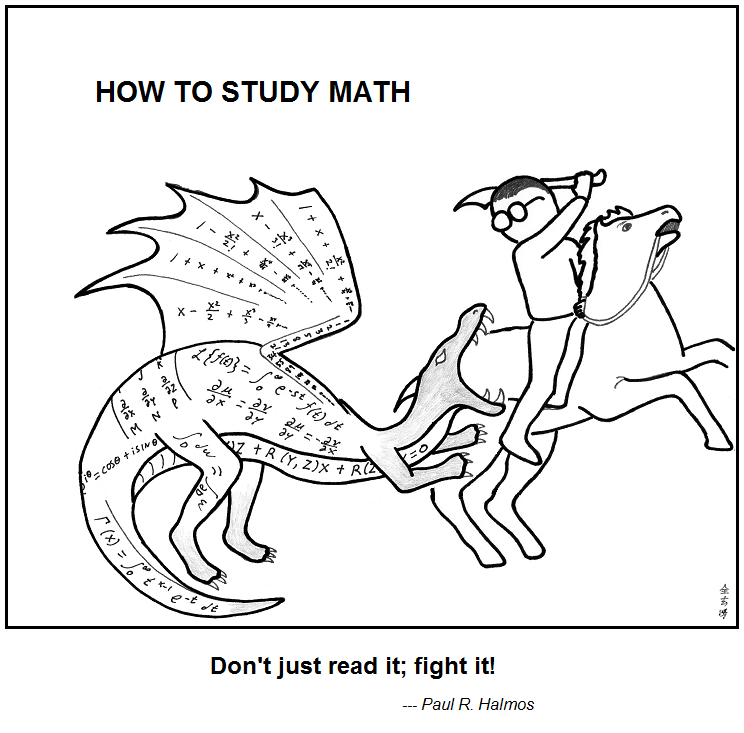
\includegraphics[width=\linewidth]{images/abstrusegoose.png}
\end{image}%
\tcblower
\end{figureptx}%
\begin{quote}%
\nopagebreak\par%
\hfill\textemdash{}{\setlength{\tabcolsep}{0pt}\begin{tabular}[t]{l@{}}
Paul Halmos
\end{tabular}}\\\par
\emph{Don't just read it; fight it!} Ask your own questions, look for your own examples, discover your own proofs. Is the hypothesis necessary? Is the converse true?\textellipsis{} Where does the proof use the hypothesis?%
\end{quote}
\end{subsubsectionptx}
\end{subsectionptx}
%
%
\typeout{************************************************}
\typeout{Subsection 2.2 Coursework and evaluation}
\typeout{************************************************}
%
\begin{subsectionptx}{Coursework and evaluation}{}{Coursework and evaluation}{}{}{x:subsection:section-evaluation}
%
%
\typeout{************************************************}
\typeout{Subsubsection 2.2.1 What are your expectations of students?}
\typeout{************************************************}
%
\begin{subsubsectionptx}{What are your expectations of students?}{}{What are your expectations of students?}{}{}{g:subsubsection:idm140338498536272}
%
\begin{itemize}[label=\textbullet]
\item{}I expect you to make your best effort to arrive prepared for each class. I'm also aware that this is not always possible.%
\item{}I expect quality writing: complete sentences, proper use of notation, and clear exposition. I don't expect this right away, but I do expect you to work at improving.%
\item{}I expect you to treat your classmates with respect, and to contribute to group activities to the best of your ability.%
\item{}I expect you to ask for help when you need it. (Everyone does at some point.)%
\end{itemize}
%
\end{subsubsectionptx}
%
%
\typeout{************************************************}
\typeout{Subsubsection 2.2.2 Thanks, but what I really meant is, how do I earn my grade?}
\typeout{************************************************}
%
\begin{subsubsectionptx}{Thanks, but what I really meant is, how do I earn my grade?}{}{Thanks, but what I really meant is, how do I earn my grade?}{}{}{g:subsubsection:idm140338498421488}
Oh, right. The most frequently asked question of all. There are several different evaluation components that contribute to your grade:%
\begin{tableptx}{\textbf{Relative weights of graded activities for Math 3410}}{x:table:table-evaluation}{}%
\centering
\begin{tabular}{lcc}\hrulethin
Component&Number&Total Weight\tabularnewline\hrulethin
Quizzes&11&10\tabularnewline[0pt]
Assignments&8&30\tabularnewline[0pt]
Term tests&2&30\tabularnewline[0pt]
Final exam&1&30\tabularnewline\hrulethin
\end{tabular}
\end{tableptx}%
\end{subsubsectionptx}
%
%
\typeout{************************************************}
\typeout{Subsubsection 2.2.3 What is involved with each of the graded components?}
\typeout{************************************************}
%
\begin{subsubsectionptx}{What is involved with each of the graded components?}{}{What is involved with each of the graded components?}{}{}{g:subsubsection:idm140338498058896}
Here are brief descriptions of each one:%
\begin{description}
\item[{Quizzes}]We'll start each week with a short quiz (10 minutes or so). Questions will be conceptual, or check your knowledge of definitions, etc.\@. Significant computational work is unlikely.%
\item[{Assignments}]Take-home assignments will contain a mix of theory and application. You will be asked to write proofs. You will also be asked to solve computational problems. Computations can be done with the aid of a computer.%
\par
The preferred format for solutions to applied problems is the \terminology{Jupyter notebook}. All U of L students have access to the \initialism{PIMS} Jupyter hub, called \href{https://uleth.syzygy.ca}{\terminology{Syzygy}}. Jupyter notebooks will allow you to write both text and Python code. I'll provide sample code to get you started. You don't need to be a programmer. (I'm not.) You just need to learn a few commands to perform things like matrix operations.%
\item[{Tests}]There will be two term tests. \alert{Test 1} is scheduled for Thursday, October 10th. \alert{Test 2} is scheduled for Thursday, November 7th.%
\par
\emph{Note:} Thursday, November 7th is just before the Fall Break. This is preferable for me, since it gives me time to grade your second test. But it's possible all your other instructors had the same idea. If that's the case, we can hold Test 2 on Tuesday the 19th instead.%
\item[{Final Exam}]A traditional, cumulative, three-hour exam. Note that final exams are no longer scheduled according to the timetable, so the date of the final exam will not be known until sometime in October. You should plan to remain on campus for the entire exam period. The Registrar's Office \emph{will not} allow you to reschedule due to travel conflicts.%
\end{description}
%
\end{subsubsectionptx}
%
%
\typeout{************************************************}
\typeout{Subsubsection 2.2.4 How are letter grades calculated?}
\typeout{************************************************}
%
\begin{subsubsectionptx}{How are letter grades calculated?}{}{How are letter grades calculated?}{}{}{g:subsubsection:idm140338499747664}
Each of the grade components above will be assigned a numerical score. These will be added to get a score out of 100 using \hyperref[x:table:table-evaluation]{Table~\ref{x:table:table-evaluation}}. Your score out of 100 is converted into a letter grade according to the following table.%
\begin{tableptx}{\textbf{Conversion of percentage scores to letter grades in Math 3410}}{x:table:table-lettergrade}{}%
\centering
\noindent\hspace{-40pt}\begin{tabular}{llllllllllll}\hrulethin
A+&A&A-&B+&B&B-&C+&C&C-&D+&D&F\tabularnewline\hrulethin
95-100&90-94&86-89&82-85&77-81&73-76&69-72&64-68&60-63&56-59&50-55&0-49\tabularnewline\hrulethin
\end{tabular}
\end{tableptx}%
\end{subsubsectionptx}
\end{subsectionptx}
%
%
\typeout{************************************************}
\typeout{Subsection 2.3 Course policies}
\typeout{************************************************}
%
\begin{subsectionptx}{Course policies}{}{Course policies}{}{}{x:subsection:section-policy}
\begin{introduction}{}%
This section deals with questions about accommodations, missed tests, and other exceptional (yet common) cases.%
\end{introduction}%
%
%
\typeout{************************************************}
\typeout{Subsubsection 2.3.1 One of the tests conflicts with something else in my schedule. What are my options?}
\typeout{************************************************}
%
\begin{subsubsectionptx}{One of the tests conflicts with something else in my schedule. What are my options?}{}{One of the tests conflicts with something else in my schedule. What are my options?}{}{}{g:subsubsection:idm140338497728528}
If you know in advance that you will not be able to attend a test due to an ``approved absence'', like varsity athletics, a conference, tea with the Queen, etc.\@, send me an email. We will try to arrange an alternate sitting of the test. (Individual stage only.)%
\end{subsubsectionptx}
%
%
\typeout{************************************************}
\typeout{Subsubsection 2.3.2 I missed a test! What do I do? Do I get a zero?}
\typeout{************************************************}
%
\begin{subsubsectionptx}{I missed a test! What do I do? Do I get a zero?}{}{I missed a test! What do I do? Do I get a zero?}{}{}{g:subsubsection:idm140338497773296}
Contact me \initialism{ASAP} to make alternate arrangements. Make-up tests are possible, but only if you contact me in time. (Advance notice is preferred when possible.) If no arrangements can be made, we will meet to discuss adjustments to your grading scheme.%
\end{subsubsectionptx}
%
%
\typeout{************************************************}
\typeout{Subsubsection 2.3.3 Do I need a doctor's note?}
\typeout{************************************************}
%
\begin{subsubsectionptx}{Do I need a doctor's note?}{}{Do I need a doctor's note?}{}{}{g:subsubsection:idm140338497666800}
No. This wastes health care resources and your time. Just email me to say you were sick. However, if you miss more than one test due to illness, we'll need to meet to discuss how to adjust your grade.%
\end{subsubsectionptx}
%
%
\typeout{************************************************}
\typeout{Subsubsection 2.3.4 What if my car breaks down?}
\typeout{************************************************}
%
\begin{subsubsectionptx}{What if my car breaks down?}{}{What if my car breaks down?}{}{}{g:subsubsection:idm140338499872352}
Same thing, for this, or other circumstances beyond your control. Send me an email, and we'll sort something out. But if there's a snowstorm forecast for the night before, maybe don't plan a trip to Calgary.%
\end{subsubsectionptx}
%
%
\typeout{************************************************}
\typeout{Subsubsection 2.3.5 I'm on one of the Pronghorns teams.}
\typeout{************************************************}
%
\begin{subsubsectionptx}{I'm on one of the Pronghorns teams.}{}{I'm on one of the Pronghorns teams.}{}{}{g:subsubsection:idm140338497628192}
Good for you!%
\par
Oh, you probably have some scheduling issues. Your coach should be providing you with a letter. Plan to meet with me during office hours one day and we'll sort something out.%
\end{subsubsectionptx}
%
%
\typeout{************************************************}
\typeout{Subsubsection 2.3.6 I receive learning accommodations. What arrangements can I make?}
\typeout{************************************************}
%
\begin{subsubsectionptx}{I receive learning accommodations. What arrangements can I make?}{}{I receive learning accommodations. What arrangements can I make?}{}{}{g:subsubsection:idm140338499882800}
First, make sure that you have registered with the University's \href{https://www.uleth.ca/ross/accommodated-learning-centre}{Accommodated Learning Centre}. If you have exam accommodations, you'll need to schedule your exams with them. No need to let me know: they'll contact me to request a copy of your exam.%
\par
If you require any in-class accommodations, or if there are any adjustments I can make to facilitate your learning, please do not hesitate to get in touch with me. All students deserve an equal opportunity to learn.%
\end{subsubsectionptx}
%
%
\typeout{************************************************}
\typeout{Subsubsection 2.3.7 Do we get to have calculators for the tests?}
\typeout{************************************************}
%
\begin{subsubsectionptx}{Do we get to have calculators for the tests?}{}{Do we get to have calculators for the tests?}{}{}{g:subsubsection:idm140338497483312}
Yes. Maybe even a computer, if I decide that I want to include computational problems, and I can guarantee that everyone has access to a computer. (You can safely assume that if a computer \emph{is} allowed, someone will be watching you like a hawk to make sure you don't use it inappropriately.)%
\end{subsubsectionptx}
%
%
\typeout{************************************************}
\typeout{Subsubsection 2.3.8 Life intervened and I can't keep up this week. What do I do?}
\typeout{************************************************}
%
\begin{subsubsectionptx}{Life intervened and I can't keep up this week. What do I do?}{}{Life intervened and I can't keep up this week. What do I do?}{}{}{g:subsubsection:idm140338497505872}
Send me an email. Extensions are usually granted as long as they're granted ahead of time. Online homework extensions need to be in place before solutions become available. See me if you're having trouble, or take a look at the other resources mentioned in \hyperref[x:subsubsection:question-help]{Question~\ref{x:subsubsection:question-help}}.%
\end{subsubsectionptx}
%
%
\typeout{************************************************}
\typeout{Subsubsection 2.3.9 I missed class. What do I do?}
\typeout{************************************************}
%
\begin{subsubsectionptx}{I missed class. What do I do?}{}{I missed class. What do I do?}{}{}{g:subsubsection:idm140338497525072}
If it's a one-time thing, don't worry about it. Drop by during office hours if you need to catch up. If circumstances are conspiring to keep you from class on a regular basis, please meet with me to come up with a plan to get you through the course.%
\end{subsubsectionptx}
%
%
\typeout{************************************************}
\typeout{Subsubsection 2.3.10 Is there anything else I need to know?}
\typeout{************************************************}
%
\begin{subsubsectionptx}{Is there anything else I need to know?}{}{Is there anything else I need to know?}{}{}{g:subsubsection:idm140338497535744}
Students are expected to abide by the policies and regulations as laid out in the \href{https://www.uleth.ca/ross/academic-calendar}{Academic Calendar}. This includes the University's policies on plagiarism and academic misconduct. In Math 3410, this more or less amounts to not copying on the tests, and not getting someone else (including a website) to do your homework for you.%
\end{subsubsectionptx}
%
%
\typeout{************************************************}
\typeout{Subsubsection 2.3.11 I have a question that isn't answered here. How do I contact you?}
\typeout{************************************************}
%
\begin{subsubsectionptx}{I have a question that isn't answered here. How do I contact you?}{}{I have a question that isn't answered here. How do I contact you?}{}{}{x:subsubsection:section-communication}
Short answer: you can \href{mailto:sean.fitzpatrick@uleth.ca}{send me an email}. There are a few caveats, however:%
\begin{itemize}[label=\textbullet]
\item{}First, check the course page (and the announcements forum) on Moodle. Any information I need to communicate to the class will be posted on Moodle, or emailed to the class as an announcement via Moodle.%
\item{}Is the question about homework? Email is not a good medium for discussing math. Your best option is to ask me in person. If that doesn't work, we have a class discussion forum, on \href{https://piazza.com}{Piazza.com}. You'll be able to access the forum via Moodle.%
\end{itemize}
%
\end{subsubsectionptx}
%
%
\typeout{************************************************}
\typeout{Subsubsection 2.3.12 I sent you an email. Why haven't you answered it yet?}
\typeout{************************************************}
%
\begin{subsubsectionptx}{I sent you an email. Why haven't you answered it yet?}{}{I sent you an email. Why haven't you answered it yet?}{}{}{g:subsubsection:idm140338497380992}
Here's a short troubleshooting guide:%
\begin{itemize}[label=\textbullet]
\item{}Your email was not sent from a ULeth account and had no subject line: It went to my spam folder.%
\item{}Your email sent between 10 pm and 6 am: I'm asleep. I'll answer when I get to work in the morning.%
\item{}Your email sent during office hours: I'm busy helping the students who are here in person. Consider dropping by yourself.%
\item{}Your email asked for help on a specific homework problem: Direct your question to the online forum.%
\item{}Your email was about something already addressed in this \initialism{FAQ}, and I need time to come up with a polite reply.%
\end{itemize}
%
\end{subsubsectionptx}
\end{subsectionptx}
\end{sectionptx}
%
%
\pagebreak
\typeout{************************************************}
\typeout{Section 3 Course topics}
\typeout{************************************************}
%
\begin{sectionptx}{Course topics}{}{Course topics}{}{}{x:section:section-schedule}
The following table provides a list of the topics we'll attempt to cover in Math 3410, along with the dates I think we'll get to them, and where they can be found in the textbook.%
\begin{tableptx}{\textbf{Math 3410 topics schedule for Fall 2019}}{x:table:table-schedule}{}%
\centering
\begin{tabular}{lll}
September 5&Introduction and review&5.1  \textendash{}  5.4\tabularnewline[0pt]
September 10&Vector spaces&6.1\tabularnewline[0pt]
September 12&Subspaces&6.2\tabularnewline[0pt]
September 17&Span and independence&6.3\tabularnewline[0pt]
September 19&Basis and dimension&6.4\tabularnewline[0pt]
September 24&Applications&6.5 \textendash{} 6.6\tabularnewline[0pt]
September 26&Linear transformations&7.1\tabularnewline[0pt]
October 1&Kernel and image&7.2\tabularnewline[0pt]
October 3&Inverses and isomorphisms&7.3\tabularnewline[0pt]
October 8&Applications&7.4  \textendash{}  7.5\tabularnewline[0pt]
October 10&Test 1&6.1 \textendash{} 7.3\tabularnewline[0pt]
October 15&Inner products&10.1\tabularnewline[0pt]
October 17&Orthogonality&5.3, 10.2\tabularnewline[0pt]
October 22&Complement and projection&8.1\tabularnewline[0pt]
October 24&Diagonalization&8.2, 10.3\tabularnewline[0pt]
October 29&QR decomposition&8.3, 8.4\tabularnewline[0pt]
October 31&Singluar value decomposition&8.5, 8.6\tabularnewline[0pt]
November 5&Complex matrices&8.7\tabularnewline[0pt]
November 7&Test \#2&10.1 \textendash{} 10.3, 8.1 \textendash{} 8.6\tabularnewline[0pt]
November 19&Change of basis&9.1\tabularnewline[0pt]
November 21&Similarity&9.2\tabularnewline[0pt]
November 27&Direct sums&9.3\tabularnewline[0pt]
November 29&Triangular matrices&11.1\tabularnewline[0pt]
December 4&Jordan form&11.2
\end{tabular}
\end{tableptx}%
\end{sectionptx}
\end{document}